\documentclass[12pt,a4paper]{report}

\usepackage[T1]{fontenc}
\usepackage[utf8]{inputenc}
\usepackage[brazilian]{babel}
\usepackage{hyphenat}
\usepackage{amssymb}
\usepackage{amsmath}
\usepackage{graphicx}
\usepackage{float}
\graphicspath{ {images/} }
\usepackage{biblatex}
\usepackage{csquotes}
\addbibresource{bibliography.bib}
\usepackage{caption}

\newcommand{\I}{{\mathrm{i}\mkern1mu}}
\newcommand{\euler}{{\mathrm{e}\mkern1mu}}

\title{Desenvolvimento de uma plataforma interativa de processamento de sinais}
\author{Mateus Fuga Osmarin}
\date{\today}

\begin{document}
\maketitle
\tableofcontents
\begin{abstract}
  Este trabalho trata do desenvolvimento de uma plataforma interativa de processamento de sinais.
  A partir de uma interface gráfica, é possível realizar o projeto de filtros digitais tanto do tipo
  IIR quanto FIR, utilizando técnicas clássicas da literatura. O sistema busca endereçar a dificuldade
  de visualização no aprendizado do tópico de processamento de sinais, fazendo-se uma ferramenta didática
  alternativa.

  \textbf{Palavras-chave}: Processamento de sinais. Projeto de filtros digitais. Visualização. Python.
\end{abstract}
\chapter{Introdução}
  A disciplina de processamento de sinais é uma área ampla que permite entender e tratar matematicamente
  sinais, transformando-os segundo as necessidades envolvidas na sua aplicação. Majoritariamente, encontra-se
  no dia-a-dia sinais de natureza contínua no tempo, como a temperatura de um corpo, o som de um instrumento
  musical ou a velocidade de um automóvel. Ainda, existem sinais de natureza inerentemente discreta no tempo,
  como é o caso do preço de uma ação, as temperaturas máxima e mínima diárias de uma cidade ou o número diário
  de novos casos de COVID-19. Entretanto, é importante ressaltar que mesmo sinais de natureza contínua  podem
  ser tratados de forma discreta por meio de procedimentos de amostragem adequados. Dessa forma, o processamento
  digital de sinais é uma técnica que pode ser aplicada a uma infinidade de casos.

  Diante da generalidade envolvida, tem-se também um nível de abstração elevado no formalismo matemático que
  fundamenta a disciplina, o que resulta em dificuldades no aprendizado dessa importante área. Nesse sentido,
  a utilização de ferramentas como a FDATool do MATLAB traz benefícios tanto de produtividade para profissionais
  da área como facilitam o aprendizado para estudantes do tópico, por abordar de forma visual e intuitiva o
  projeto de filtros digitais. Utilizando esse tipo de ferramenta, pode-se variar parâmetros de projeto e
  visualizar o comportamento dos sistemas projetados de forma eficiente e facilitada, com gráficos que exibem
  as principais características do processo. Contudo, o MATLAB se trata de um software pago e, não obstante,
  tem-se observado um aumento crescente no interesse pela linguagem de programação Python por estudantes e
  profissionais da área, dada a grande quantidade de bibliotecas disponíveis para todo tipo de problemas.

  Dessa forma, o presente trabalho tem como objetivo o desenvolvimento de um software livre para projeto de
  filtros digitais utilizando a linguagem de programação Python, construindo uma interface gráfica amigável em
  GTK para aumento de produtividade e facilitar o aprendizado na área de processamento de sinais, contando com
  uma revisão de conceitos importantes a servir como referência para utilização do sistema.
\chapter{Referenciais teóricos}
\section{Sinais}
  Em essência, um sinal é algo que contém alguma informação, geralmente sobre o estado de um sistema físico
  \cite{oppenheim}. Podemos definir matematicamente um sinal como sendo uma função, de uma ou mais variáveis
  independentes. A natureza dessas variáveis é diversa, sendo o tempo e o espaço as mais usuais. O som é um
  exemplo de sinal temporal, enquanto a temperatura em uma sala ao longo do dia se refere a um sinal espacial e
  temporal. No decorrer deste trabalho, serão considerados sinais de uma variável, sendo tomada como temporal
  por convenção, mas a teoria é igualmente válida para outros domínios.

  Um sinal contínuo no tempo é definido como sendo uma função do tempo definida para todos os instantes:
  \begin{equation}
    x = x(t), t \in \mathbb{R}
  \end{equation}
  A figura \ref{fig:continuous} mostra um exemplo de sinal contínuo no tempo.
  \begin{figure}
    \caption{Sinal contínuo no tempo}
    \centering
    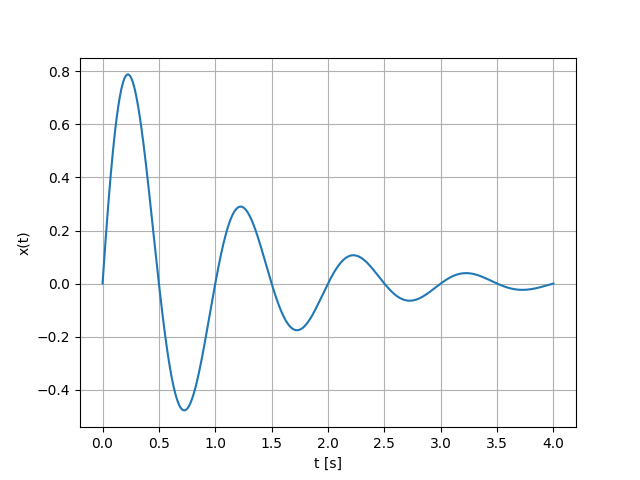
\includegraphics[width=0.75\textwidth]{continuous}
    \label{fig:continuous}
    \caption*{Fonte: Autoria própria}
  \end{figure}

  Um sinal discreto no tempo, por outro lado, é definido como uma sequência numérica:
  \begin{equation}
    x = x[n], n \in \mathbb{Z}
  \end{equation}

  Para tratar discretamente sinais contínuos no tempo, pode-se amostrar o sinal contínuo em intervalos de tempo
  igualmente espaçados:
  \begin{equation}
    x_d[n] = x_a(n T_s)
  \end{equation}
  onde $x_d$ é a versão discretizada do sinal analógico $x_a$ e $T_s$ representa o período de amostragem.
  A figura \ref{fig:discrete} mostra o sinal da figura \ref{fig:continuous} discretizado.
  \begin{figure}
    \caption{Sinal discreto no tempo}
    \centering
    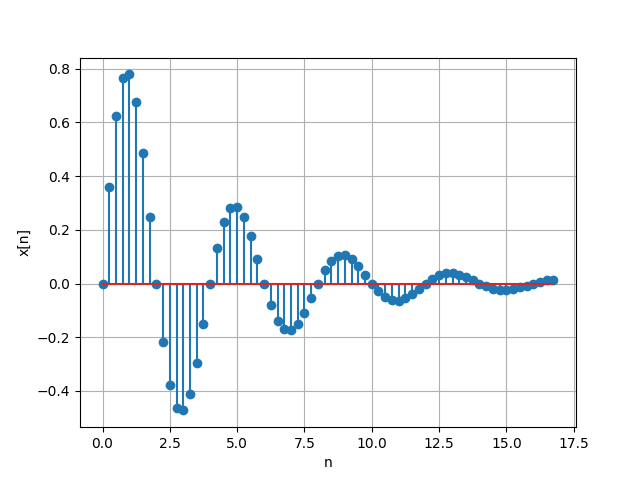
\includegraphics[width=0.75\textwidth]{discrete}
    \label{fig:discrete}
    \caption*{Fonte: Autoria própria}
  \end{figure}

  Dentre os sinais existentes, o impulso unitário ou delta de Dirac, é um dos mais importantes. Este sinal é
  definido, no caso contínuo, como:
  \begin{equation}
    \delta(t) =
      \left
      \{
      \begin{array}{rcl}
        0 & \mbox{para} & t \neq 0 \\
        \infty & \mbox{para} & t = 0
      \end{array}
      \right.
  \end{equation}
  satisfazendo a restrição
  \begin{equation}
    \int_{-\infty}^{+\infty} \delta(t) dt = 1
  \end{equation}

  Uma propriedade notória do impulso unitário é que
  \begin{equation}
    \int_{-\infty}^{+\infty} f(t) \delta(t-t_0) dt = f(t_0)
  \end{equation}
  sendo conhecida como propriedade da amostragem.

  No caso discreto, o impulso unitário é definido como:
  \begin{equation}
    \delta[n] =
      \left
      \{
      \begin{array}{rcl}
        0 & \mbox{para} & n \neq 0 \\
        1 & \mbox{para} & n = 0
      \end{array}
      \right.
  \end{equation}

  A propriedade da amostragem para o caso discreto é expressa como:
  \begin{equation}
    \sum_{n = -\infty}^{+\infty} x[n] \delta[n-n_0] = x[n_0]
  \end{equation}

\section{Transformadas de Fourier, Laplace e Z}
  Até aqui, os sinais foram descritos no domínio do tempo. É possível, no entanto, representar sinais no
  domínio da frequência através das transformações conhecidas como transformada de Fourier, transformada de
  Laplace e transformada Z. O princípio de partida é a série de Fourier, que possibilita a representação de uma
  função T-periódica como uma série de senos e cossenos ou, equivalentemente, exponenciais complexas.

  A série de Fourier é definida como:
  \begin{equation}
    x_N(t) = \sum_{n = -N}^{+N} c_n \euler^{\I \frac{2 \pi}{T} n t}
  \end{equation}
  onde
  \begin{equation}
    c_n = \frac{1}{T} \int_T x(t) \euler^{-\I \frac{2 \pi}{T} n t} dt
  \end{equation}
  são os coeficientes da série, e N é teoricamente infinito. A figura \ref{fig:fourier} mostra a expansão
  em série de Fourier do retângulo unitário para diferentes valores de N.
  \begin{figure}[H]
    \caption{Expansão em série de Fourier do retângulo unitário}
    \centering
    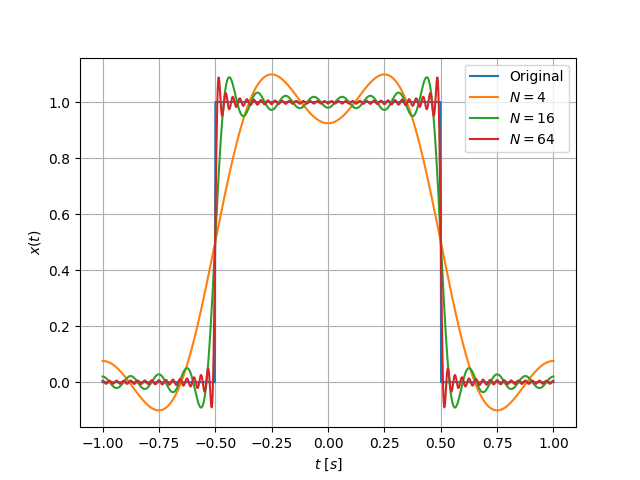
\includegraphics[width=0.75\textwidth]{fourier_series}
    \label{fig:fourier}
    \caption*{Fonte: Autoria própria}
  \end{figure}

  Para funções não-periódicas, generaliza-se a série de Fourier considerando o período como sendo infinito.
  No caso limite, tem-se:
  \begin{equation}
    x(t) = \int_{-\infty}^{+\infty} \widehat{x}(f) \euler^{\I 2 \pi f t} df
  \end{equation}
  onde
  \begin{equation}
    \widehat{x}(f) = \mathcal{F}\{x(t)\}(f) = \int_{-\infty}^{+\infty} x(t) \euler^{-\I 2 \pi f t} dt
  \end{equation}
  e $\widehat{x}(f)$ é conhecida como a transformada de Fourier de $x(t)$. Segundo esta definição, $f$ tem
  unidades de $hertz$. A figura \ref{fig:fourier_transform} mostra a transformada de Fourier do retângulo
  unitário.
  \begin{figure}[H]
    \caption{Transformada de Fourier do retângulo unitário}
    \centering
    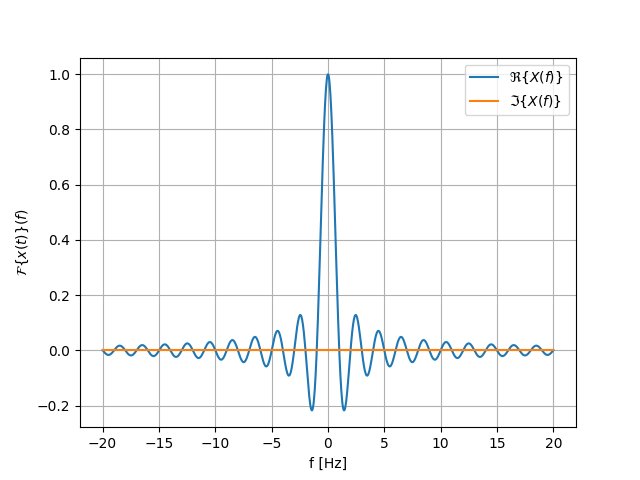
\includegraphics[width=0.75\textwidth]{fourier_transform}
    \label{fig:fourier_transform}
    \caption*{Fonte: Autoria própria}
  \end{figure}

  Ao amostrar um sinal com um período de amostragem $T$ por meio de um pente de Dirac
  \begin{equation}
    \begin{split}
      x_T(t) = &\quad x(t) \sum_{n = -\infty}^{+\infty} \delta(t - n T) \\
      = &\quad \sum_{n = -\infty}^{+\infty} x(n T) \delta(t - n T) \\
      = &\quad \sum_{n = -\infty}^{+\infty} x[n] \delta(t - n T)
    \end{split}
    \label{eq:dirac_comb}
  \end{equation}
  e aplicar a transformada de Fourier, tem-se
  \begin{equation}
    \begin{split}
      \widehat{x}_T(f) = &\quad \int_{-\infty}^{+\infty} \sum_{n = -\infty}^{+\infty}
                                x[n] \delta(t - n T) \euler^{-\I 2 \pi f t} dt
      \\ = &\quad \sum_{n = -\infty}^{\infty} x[n] \int_{-\infty}^{+\infty}
                                \delta(t - n T) \euler^{-\I 2 \pi f t} dt
      \\ = &\quad \sum_{n = -\infty}^{+\infty} x[n] \euler^{-\I 2 \pi f n T}
    \end{split}
  \end{equation}
  ao que se obtém a chamada transformada de tempo discreto de Fourier. Para obter o sinal original, a
  transformada de tempo discreto de Fourier inversa é:
  \begin{equation}
    x[n] = T \int_{1/T} \widehat{x}_T(f) \euler^{\I 2 \pi f n T} df
  \end{equation}

  A figura \ref{fig:discrete_time_fourier_transform} mostra a transformada de tempo discreto de Fourier do
  retângulo unitário.
  \begin{figure}[H]
    \caption{Transformada de tempo discreto de Fourier do retângulo unitário}
    \centering
    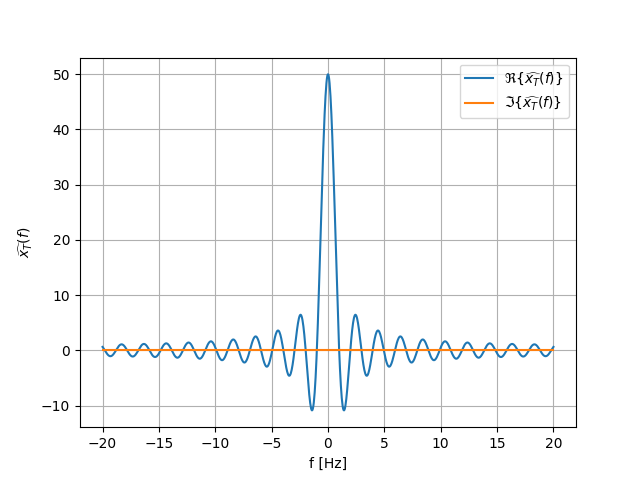
\includegraphics[width=0.75\textwidth]{discrete_time_fourier_transform}
    \label{fig:discrete_time_fourier_transform}
    \caption*{Fonte: Autoria própria}
  \end{figure}
  Nesse caso, a discretização acontece no domínio do tempo, mas a frequência ainda é contínua. Discretizando a
  transformada de tempo discreto de Fourier para $N$ amostras de um ciclo, obtém-se:
  \begin{equation}
    \begin{split}
      X[k] = &\quad \widehat{x}_T\left(\frac{k}{N T}\right)
      \\ &\quad = \sum_{n = -\infty}^{+\infty} x[n] \euler^{-\I 2 \pi \frac{k}{N T} n T}
      \\ &\quad = \sum_{n = -\infty}^{+\infty} x[n] \euler^{-\I 2 \pi \frac{k}{N} n}
    \end{split}
  \end{equation}
  o que define a transformada discreta de Fourier. Para obter o sinal original, a transformada discreta de
  Fourier inversa é:
  \begin{equation}
    x[n] = \frac{1}{N} \sum_{k = -\infty}^{+\infty} X[k] \euler^{\I 2 \pi \frac{k}{N} n}
  \end{equation}
  
  A figura \ref{fig:discrete_fourier_transform} mostra a transformada discreta de Fourier do retângulo unitário.
  \begin{figure}[H]
    \caption{Transformada discreta de Fourier do retângulo unitário}
    \centering
    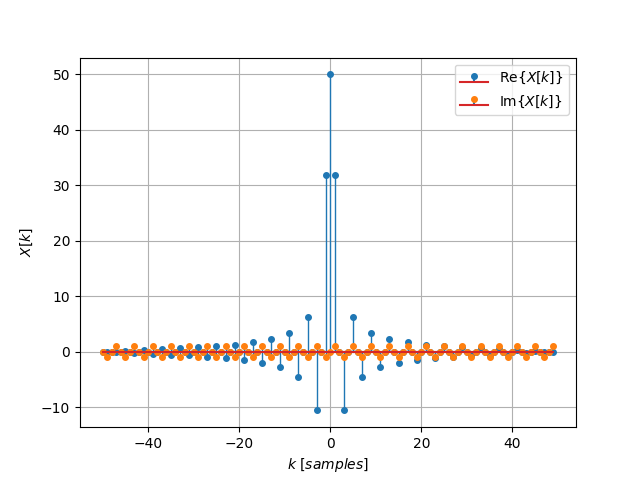
\includegraphics[width=0.75\textwidth]{discrete_fourier_transform}
    \label{fig:discrete_fourier_transform}
    \caption*{Fonte: Autoria própria}
  \end{figure}

  A transformada de Fourier pode ainda ser generalizada ao se considerar uma frequência complexa. O resultado
  é a transformada de Laplace:
  \begin{equation}
    X(s) = \mathcal{L}\{x(t)\}(s) = \int_{-\infty}^{+\infty} x(t) \euler^{-s t} dt
  \end{equation}
  onde
  \begin{equation}
    s = \sigma + \I \omega = \sigma + \I 2 \pi f
  \end{equation}

  A figura \ref{fig:laplace_transform} mostra a transformada de Laplace do retângulo unitário.
  \begin{figure}[H]
    \caption{Transformada de Laplace do retângulo unitário}
    \centering
    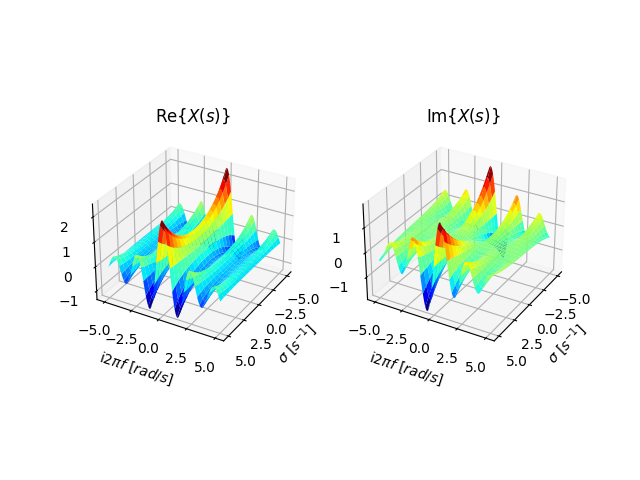
\includegraphics[width=0.75\textwidth]{laplace_transform}
    \label{fig:laplace_transform}
    \caption*{Fonte: Autoria própria}
  \end{figure}

  Nota-se também que a transformada de Laplace pode ser vista como sendo a transformada de Fourier de
  $x(t) \euler^{-\sigma t}$. Para recuperar o sinal original, a transformada de Laplace inversa é:
  \begin{equation}
    x(t) = \mathcal{L}^{-1}\{X(s)\}(t) = \frac{1}{\I 2 \pi} \lim_{T \rightarrow \infty}
    \int_{\gamma - \I T}^{\gamma + \I T} X(s) \euler^{s t} ds
  \end{equation}
  onde $\gamma$ é um número real tal que o caminho de integração esteja na região de convergência de $F(s)$.

  Novamente, amostrando um sinal por meio de um pente de Dirac \eqref{eq:dirac_comb} e aplicando
  a transformada de Laplace, tem-se
  \begin{equation}
    \begin{split}
      X_T(s) = &\quad \int_{-\infty}^{+\infty} \sum_{n = -\infty}^{+\infty} x[n] \delta(t - n T) \euler^{-s t} dt
      \\= &\quad \sum_{n = -\infty}^{+\infty} x[n] \int_{-\infty}^{+\infty} \delta(t - n T) \euler^{-s t} dt
      \\= &\quad \sum_{n = -\infty}^{+\infty} x[n] \euler^{-s n T}
    \end{split}
  \end{equation}
  da qual, ao tomar $z = \euler^{s T}$, obtém-se a transformada Z de um sinal discreto:
  \begin{equation}
    X(z) = \mathcal{Z}\{x[n]\}(z) = \sum_{n = -\infty}^{+\infty} x[n] z^{-n}, z \in \mathbb{C}
  \end{equation}

  Para recuperar o sinal original, a transformada Z inversa é:
  \begin{equation}
    x[n] = \mathcal{Z}^{-1}\{X(z)\}[n] = \frac{1}{\I 2 \pi} \oint_{\mathcal{C}} X(z) z^{n - 1} dz
  \end{equation}
  onde $\mathcal{C}$ é um caminho fechado percorrido no sentido anti-horário, contendo a origem e inteiramente
  na região de convergência de $X(z)$.

\section{Convolução}
  Dados dois sinais, é possível realizar um conjunto de operações sobre os mesmos. Dentre estas, tem-se as bem
  conhecidas operações de soma, subtração, multiplicação, divisão, derivação e integração. Em processamento
  de sinais, uma operação conhecida como convolução é muito utilizada, sendo definida por:
  \begin{equation}
    (f \ast g)(t) = \int_{-\infty}^{+\infty} f(\tau) g(t - \tau) d\tau
  \end{equation}
  para o caso contínuo e
  \begin{equation}
    (f \ast g)[n] = \sum_{k = -\infty}^{+\infty} f[k] g[n - k]
  \end{equation}
  para o caso discreto.

  Uma propriedade importante da convolução é
  \begin{equation}
    \label{eq:continuous_convolution_identity}
    x(t) \ast \delta(t) = \int_{-\infty}^{+\infty} x(\tau) \delta(t - \tau) d\tau = x(t)
  \end{equation}
  para o caso contínuo e
  \begin{equation}
    \label{eq:discrete_convolution_identity}
    x[n] \ast \delta[n] = \sum_{k = -\infty}^{+\infty} x[k] \delta[n - k] = x[n]
  \end{equation}
  para o caso discreto. Esta propriedade exprime o fato de que o impulso unitário corresponde a uma identidade
  para a convolução.

  Ainda, outra propriedade importante da convolução está em sua relação com as transformadas de Fourier, Laplace
  e Z. Tomando a transformada de Laplace como exemplo, tem-se:
  \begin{equation}
    \label{eq:convolution_theorem}
    \begin{split}
      \mathcal{L}\{(f \ast g)(t)\}(s) = &\quad \int_{t = -\infty}^{+\infty} \left[\int_{\tau = -\infty}^{+\infty}
      f(\tau) g(t - \tau) d\tau\right] \euler^{-s t} dt
      \\ = &\quad \int_{\tau = -\infty}^{+\infty} \int_{t = -\infty}^{+\infty}
      f(\tau) g(t - \tau) \euler^{-s t} dt d\tau
      \\ = &\quad \int_{\tau = -\infty}^{+\infty} f(\tau) \int_{t = -\infty}^{+\infty}
      g(t - \tau) \euler^{-s t} dt d\tau
      \\ = &\quad \int_{\tau = -\infty}^{+\infty} f(\tau) \int_{u = -\infty}^{+\infty}
      g(u) \euler^{-s(u+\tau)} du d\tau
      \\ = &\quad \int_{\tau = -\infty}^{+\infty} f(\tau) \euler^{-s \tau} d\tau
      \int_{u = -\infty}^{+\infty} g(u) \euler^{-s u} du
      \\ = &\quad \mathcal{L}\{f(t)\}(s) \mathcal{L}\{g(t)\}(s)
    \end{split}
  \end{equation}
  ou seja, no domínio da frequência a operação de convolução corresponde à multiplicação. A equação
  \ref{eq:convolution_theorem} é conhecida como teorema do convolução.

\section{Sistemas lineares e invariantes no tempo}
  Um sistema é essencialmente algo que mapeia um sinal de entrada em um sinal de saída \cite{diniz}, ou seja:
  \begin{equation}
    y(t) = \mathcal{H}\{x(t)\}
  \end{equation}
  para um sistema analógico e
  \begin{equation}
    y[n] = \mathcal{H}\{x[n]\}
  \end{equation}
  para um sistema discreto, onde $\mathcal{H}\{\cdot\}$ denota o sistema.

  Dentre todos os sistemas possíveis, tem-se classes de sistemas que são interessantes pelas propriedades que
  apresentam. Um sistema linear é um sistema que tem a propriedade:
  \begin{equation}
    \mathcal{H}\{a x_1(t) + b x_2(t)\} = a \mathcal{H}\{x_1(t)\} + b \mathcal{H}\{x_2(t)\}
  \end{equation}
  para o caso contínuo e
  \begin{equation}
    \mathcal{H}\{a x_1[n] + b x_2[n]\} = a \mathcal{H}\{x_1[n]\} + b \mathcal{H}\{x_2[n]\}
  \end{equation}
  para o caso discreto. Sistemas com essa propriedade tem a característica de, por exemplo, ao se dobrar a
  amplitude da entrada, dobrar-se também a amplitude da saída.

  Um sistema invariante no tempo é um sistema que tem a propriedade:
  \begin{equation}
    \mathcal{H}\{x(t)\} = y(t) \Leftrightarrow \mathcal{H}\{x(t - t_0)\} = y(t - t_0)
  \end{equation}
  para o caso contínuo e
  \begin{equation}
    \mathcal{H}\{x[n]\} = y[n] \Leftrightarrow \mathcal{H}\{x[n - n_0]\} = y[n - n_0]
  \end{equation}
  para o caso discreto. Sistemas com essa propriedade tem a característica de ao se atrasar a entrada, atrasar-se
  também a saída pela mesma quantidade.

  Sistemas que são lineares e invariantes no tempo podem ser tratados matemáticamente de forma generalizada como
  se segue. Sendo $\mathcal{H}\{\cdot\}$ um sistema linear e invariante no tempo, e como, de acordo com as
  equações \ref{eq:continuous_convolution_identity} e \ref{eq:discrete_convolution_identity}, sinais podem ser
  representados por uma convolução com o impulso unitário, tem-se
  \begin{equation}
    \label{eq:continuous_system_convolution}
    \begin{split}
      y(t) = &\quad \mathcal{H}\{x(t) \ast \delta(t)\}
      = \mathcal{H}\{\int_{-\infty}^{+\infty} x(\tau) \delta(t - \tau) d\tau\}
      \\ = &\quad \int_{-\infty}^{+\infty} x(\tau) \mathcal{H}\{\delta(t - \tau)\} d\tau
      \\ = &\quad \int_{-\infty}^{+\infty} x(\tau) h(t - \tau) d\tau
      \\ = &\quad x(t) \ast h(t)
    \end{split}
  \end{equation}
  para o caso contínuo e
  \begin{equation}
    \label{eq:discrete_system_convolution}
    \begin{split}
      y[n] = &\quad \mathcal{H}\{x[n] \ast \delta[n]\}
      = \mathcal{H}\{\sum_{k = -\infty}^{+\infty} x[k] \delta[n - k]\}
      \\ = &\quad \sum_{k = -\infty}^{+\infty} x[k] \mathcal{H}\{\delta[n - k]\}
      \\ = &\quad \sum_{k = -\infty}^{+\infty} x[k] h[n - k]
      \\ = &\quad x[n] \ast h[n]
  \end{split}
  \end{equation}
  para o caso discreto. Nas equações \ref{eq:continuous_system_convolution} e
  \ref{eq:discrete_system_convolution}, $h(t)$ e $h[n]$ representam a resposta do sistema a um impulso unitário.
  Assim, um sistema linear e invariante no tempo pode ser descrito totalmente por sua resposta ao impulso.

  No domínio da frequência, o teorema da convolução \ref{eq:convolution_theorem} fornece:
  \begin{equation}
    Y(s) = \mathcal{L}\{x(t) \ast h(t)\} = X(s) H(s)
  \end{equation}
  para um sistema analógico e
  \begin{equation}
    Y(z) = \mathcal{Z}\{x[n] \ast h[n]\} = X(z) H(z)
  \end{equation}
  para um sistema discreto. Chama-se $H(s)$ e $H(z)$ a função de transferência do sistema $\mathcal{H\{\cdot}\}$.
\section{Filtros digitais}
  Em geral, um filtro digital é um sistema discreto. Neste trabalho serão abordados filtros digitais lineares e
  invariantes no tempo.

  Filtros não-recursivos são caracterizados por uma equação de diferenças do tipo:
  \begin{equation}
    y[n] = \sum_{k = 0}^{M} b_k x[n - k]
  \end{equation}
  onde os coeficientes $b_k$ estão diretamente relacionados a resposta ao impulso do sistema, ou seja,
  $b_k = h[k]$. Aplicando a transformada Z, tem-se que a função de transferência do sistema é dada por:
  \begin{equation}
    H(z) = \frac{Y(z)}{X(z)} = \sum_{k = 0}^{M} b_k z^{-k}
  \end{equation}
  Devido ao fato de a resposta ao impulso deste sistema ser de duração finita, filtros não-recursivos são também
  conhecidos como filtros de resposta ao impulso finito (FIR, do inglês \textit{finite impulse response}).

  Filtros recursivos, por outro lado, são caracterizados por uma equação de diferenças do tipo:
  \begin{equation}
    y[n] = \sum_{k = 0}^{M} b_k x[n - k] - \sum_{k = 1}^{N} a_k y[n - k]
  \end{equation}
  Aplicando a transformada Z, tem-se
  \begin{equation}
    Y(z) = \sum_{k = 0}^{M} b_k X(z) z^{-k} - \sum_{k = 1}^{N} a_k Y(z) z^{-k}
  \end{equation}
  de onde, ao se rearranjar, obtem-se
  \begin{equation}
    Y(z) \left( 1 + \sum_{k = 1}^{N} a_k z^{-k} \right) = X(z) \left( \sum_{k = 0}^{M} b_k z^{-k} \right)
  \end{equation}
  ou seja,
  \begin{equation}
    H(z) = \frac{Y(z)}{X(z)} = \frac{\sum_{k = 0}^{M} b_k z^{-k}}{1 + \sum_{k = 1}^{N} a_k z^{-k}}
  \end{equation}
  é a função de transferência do sistema. Filtros recursivos, pelo fato de que a saída do sistema depende de
  saídas passadas, apresentam uma resposta ao impulso de duração infinita, dessa forma são também conhecidos como
  filtros de resposta ao impulso infinito (IIR, do inglês \textit{infinite impulse response}).
\chapter{Resultados}
\chapter{Considerações finais}
\printbibliography
\end{document}
